\documentclass[conference]{IEEEtran}

\usepackage{amsmath,amsthm,amssymb}
\usepackage{graphicx}
\usepackage{subfigure}

\usepackage{url}
\usepackage{cite}

% correct bad hyphenation here
\hyphenation{op-tical net-works semi-conduc-tor}

\begin{document}

\title{Traf: A Camera Based System for Traffic Flow Analysis}
\maketitle
\author{fsb}

\begin{abstract}

In this paper, we present a camera based system(CBS-TFM) to count automotive vehicles for traffic flow analysis use.  The system employs the method of background subtraction by comparing differences between foreground and background. The background model is initialed by averaging first 50 frames, and adapted to environment change by introducing an adapting parameter $\lambda$. Compared to state-of-art method, it is more robust, adaptive and economical.

\end{abstract}


%--------------------------------------------------------------------------------
% what and why ?
\section{Introduction}

%================================================================================

% how?
\section{System Design}
	\subsection{Overview}
	The system consists of 3 main modules, video collector, vehicle counter and flow analyzer as Fig \ref{sysDiagram}. Video collector is designed to collect the original video sources and transform them into a unified format for further use. Flow analyzer is designed to calculate the result and provide suggestion for traffic use. The vehicle counter is the core module of the system, which further divided into 4 steps as, detector, tracker, follower and generator. 
	
	\begin{figure}[!h]
	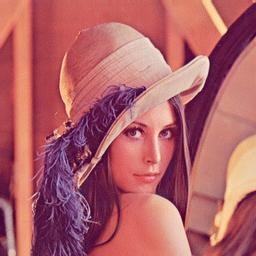
\includegraphics[width=0.8\linewidth]{lena.jpg} 
	\caption{System diagram}
	\label{sysDiagram}
	\end{figure}
	
	%============================================================================
	\subsection{Background Subtraction}
	
	\subsection{Background Model}
	\subsection{Motion Detection and Tracking}
	\subsection{Traffic Flow Analysis}
	
	
	
% compare and check	
\section{Implementation and Evaluation}
	\subsection{Setup}
	\subsection{Methodology}
	\subsection{Result}



\section{Conclusion}


\end{document}